\chapter{基于根轨迹的校正}

\section{基本思想}

\subsection{性能指标的转换}

当性能指标以时域形式给出的时候，适合采用根轨迹法设计串联校正装置，给出的时域指标可能如下：
\begin{enumerate}
    \item 阻尼比$\xi$
    \item 自然振荡频率$\omega_n$
    \item 最大超调量$\sigma_p$
    \item 调整时间$t_s$
\end{enumerate}

设计时一般根据性能指标要求确定闭环主导极点，设计校正装置，使校正后的根轨迹通过期望的闭环主导极点

如果给定的期望指标是阻尼比和自然振荡频率，则闭环主导极点为：
\begin{equation*}
    s_{1,2} = - \xi \omega_n \pm j \omega_n \sqrt{1 - \xi^2}
\end{equation*}

如果给定超调量和调节时间，则可以通过以下的式子先算出期望的阻尼比和自然振荡频率，再算出闭环主导极点：
\begin{equation*}
    \begin{split}
        \sigma \% &= e^{-\frac{\pi \xi}{\sqrt{1-\xi^2}}}  \times 100 \%     \\
        t_s &= \frac{3.5}{\xi \omega_n}
    \end{split}
\end{equation*}

\subsection{零极点对根轨迹的影响}

零点对于根轨迹的影响如下图所示：
\begin{center}
    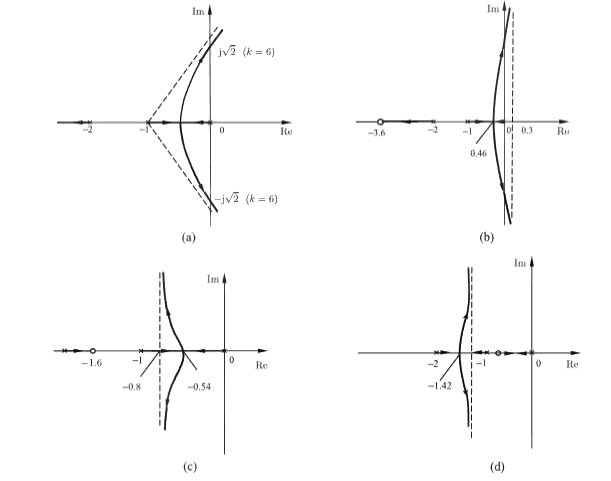
\includegraphics[width = .5\textwidth]{note/root locus correction/figure/1.png}
\end{center}
从图上可以看出添加一个零点可以使根轨迹向左或者右移动，或者使根轨迹反转

极点对于根轨迹的影响如下图所示：
\begin{center}
    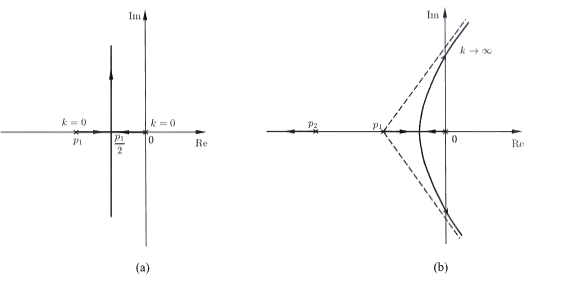
\includegraphics[width = .6\textwidth]{note/root locus correction/figure/2.png}
\end{center}

从图上可以看出添加一个极点可以使根轨迹向右移动

\subsection{超前环节}
超前环节的传递函数为
\begin{equation*}
    G_c(s) = K_c \frac{s-z_c}{s-p_c}  \quad  p_c < z_c < 0
\end{equation*}
引入超前环节之后相当于给原开环系统补充了一个零点和一个极点，同时超前环节会产生一个幅角：
\begin{equation*}
    \varphi_c = \varphi_z - \varphi_p > 0
\end{equation*}
$\varphi_c$不宜太大，否则难以实现

\textbf{超前环节会使系统根轨迹向左移动}

同时，引入超前环节相当于引入了一对开环偶极子，在加入偶极子之后，系统的开环增益发生了变化，适当选取偶极子可以增加系统的静态性能

\section{超前校正环节设计}

我们通过以下步骤，基于根轨迹进行超前校正的设计
\begin{enumerate}
    \item 根据性能指标要求，确定系统闭环主导极点$s_1$的期望位置
    \item 画出未校正系统的根轨迹，如果根轨迹通过闭环主导极点的期望位置，则简单调整开环增益即可产生期望的闭环极点；如果闭环主导极点的期望位置在根轨迹的左侧，则采用超前校正
    \item 对于期望的闭环主导极点$s_1$，按下面的式子确定超前校正环节应产生的幅角$\varphi$
    \begin{equation*}
        \varphi = (2l+1) 180^\circ - \angle G_0(s_1)
    \end{equation*}
    \item 按照下面式子确定超前校正环节的零点和极点：
    \begin{equation*}
        \angle(s_1-z_c) - \angle(s_1-p_c) = \varphi
    \end{equation*}
    \item 根据根轨迹幅值条件，按照下式确定超前校正环节的增益$K_c$
    \begin{equation*}
        K_c = \frac{\left\lvert z_c \right\rvert \left\lvert s_1 - p_c \right\rvert  }{\left\lvert G_0(s_1) \right\rvert \left\lvert p_c \right\rvert \left\lvert s_1 - z_c \right\rvert  }
    \end{equation*}
    进而确定超前校正环节的传递函数为：
    \begin{equation*}
        G_c(s) = K_c \alpha  \frac{s- z_c}{s - p_c}
    \end{equation*}
    \item 对于设计好的串联校正环节，检查校正后系统的动态性能指标是否满足设计要求。如果不满足，则需要调整主导极点的位置，重复上述设计过程
\end{enumerate}

对于超前校正环节零极点的确定，我们有以下几种方式：
\begin{enumerate}
    \item 给定具阻尼角为$\theta$的主导极点$s_1$，若超前环节在$s_1$处提供的超前角为$\varphi$，则超前环节的一组零极点由下式确定：
    \begin{equation*}
        \begin{cases}
            p_c &= -\left\lvert s_1 \right\rvert \frac{\cos \frac{1}{2}(\varphi - \theta)}{\cos \frac{1}{2} (\theta + \varphi)}  \\
            z_c &= -\left\lvert s_1 \right\rvert \frac{\cos \frac{1}{2}(\varphi + \theta)}{\cos \frac{1}{2} (\varphi - \theta)}
        \end{cases}
    \end{equation*}
    \item 给定复平面第二象限的点$s_1$和角度$\varphi$，而$p_c < z_c$是负实轴上使$\angle z_c s_1 p_c = \varphi$的两个动点。令$\angle z_c O s_1 = \theta$，则当$\angle O s_1 z_c = \frac{1}{2} (180^\circ - \theta -\varphi)$时，比值$\alpha = \frac{\left\lvert p_c \right\rvert }{\left\lvert z_c \right\rvert }$最小，且最小值$\alpha_{min}$为
    \begin{equation*}
        \alpha_{min} = 1 + \frac{2 \sin \theta \sin \varphi}{\cos (\theta + \varphi) + 1}
    \end{equation*}
    \item 幅值确定法：首先我们可以根据以下的式子算出$\angle z_c s_1 O = \eta $：
    \begin{equation*}
        \begin{split}
            \frac{1}{\tan \eta} &= \alpha \frac{\left\lvert s_1 - z_c \right\rvert}{\left\lvert s_1 - p_c \right\rvert } \frac{1}{\sin \varphi} - \frac{1}{\tan \varphi} \\
            &\alpha \frac{\left\lvert s_1 - z_c \right\rvert}{\left\lvert s_1 - p_c \right\rvert } = \frac{M}{k} \\
            M &= \frac{\left\lvert s_1^v \right\rvert \prod_{i=1}^{n-v}\left\lvert s_1 - p_i \right\rvert}{\prod_{j=1}^{m}\left\lvert s_1 - z_j \right\rvert}
        \end{split}
    \end{equation*}
    在算出$\eta$之后可以由角度关系求得：
    \begin{equation*}
        \begin{split}
            \left\lvert z_c \right\rvert &= \omega_n \frac{\sin \eta}{\sin \delta} \\
            \left\lvert p_c \right\rvert &= \omega_n \frac{\sin (\theta + \eta)}{\sin (\delta - \varphi)} \\
        \end{split}
    \end{equation*}
\end{enumerate}

\subsection{迟后校正环节设计}

我们可以通过以下步骤，设计基于根轨迹的迟后校正：
\begin{enumerate}
    \item 用原系统的开环传递函数$G_0(s)$做出原系统的根轨迹，确定调整开环增益可以使原系统的动态性能满足设计指标
    \item 在原系统的根轨迹上确定闭环主导极点$s_1$，并求出点$s_1$对应的开环增益$K_0$
    \item 根据控制系统的设计要求，求出满足稳态误差设计指标的开环增益$K$，即校正以后应有的开环增益
    \item 为了使点$s_1$的开环增益$K_0$增大到$K$，则有：
    \begin{equation*}
        \beta = \frac{K}{K_0}
    \end{equation*}
    按照串联迟后校正的条件，极点$p_c$和零点$z_c$应充分接近并靠近原点，按照
    \begin{equation*}
        \beta = \frac{z_c}{p_c}
    \end{equation*}
    可以确定校正环节的零极点值。至此，串联迟后校正环节的参数全部计算完成
    \item 绘制出校正后的根轨迹图，检验系统的动态性能指标和静态稳态性能指标
\end{enumerate}

\subsection{迟后-超前校正环节的设计}

我们可以通过以下步骤，设计基于根轨迹的迟后-超前校正环节：
\begin{enumerate}
    \item 根据期望性能指标要求，确定满足要求的闭环主导极点的候选区域
    \item 确定超前部分：作出校正前系统的根轨迹。若根轨迹未穿过候选区域，则修改初选期望闭环出到极点的位置。合理选择超前校正零极点，使其穿过期望主导极点
    \item 校验系统响应动态性能是否满足要求，不满足则可适当右移校正环节的零点和（或）左移其极点，使系统根轨迹进一步左移，绘制响应根轨迹，并重新选择裕度更大的闭环系统主导极点。
    \item 确定迟后部分：对新选主导极点，按幅值条件求出校正后系统的根轨迹增益$k$以及静态误差系数，检验系统稳态精度是否满足要求。若不满足要求，则根据稳态误差要求确定迟后校正零极点位置
    \item 迟后校正后，原主导极点位置可能发生变化。此时，应绘制迟后超前校正后系统根轨迹，判断系统动、静态性能是否满足要求。
\end{enumerate}

\subsection{反馈校正的设计}

我们可以通过以下步骤，设计基于根轨迹的局部反馈校正：
\begin{enumerate}
    \item 做出未进行局部反馈的原系统的根轨迹。
    \item 求出满足设计要求的闭环主导极点的位置$s_1$和$s_2$
    \item 在系统的开环极点中，找出系统改变位置的开环极点$p_c$，当改变$p_c$的位置时，可以使根轨迹通过$s_1$和$s_2$点
    \item 检验围绕$p_c$是否可以建立局部反馈。即在实际问题中，$p_c$所在的原件的输出变量是否可以测量；$p_c$所在原件的输入变量是否可以实现相加
    \item 为使闭环主导极点达到$s_1$和$s_2$，按照根轨迹的复制条件，求出极点$p_c$的希望位置$\overline{p}_c$
    \item 求出使小闭环的闭环极点成为$\overline{p}_c$的条件，从而确定小闭环的参数
    \item 对于大闭环，求出主导极点$s_1$和$s_2$所对应的开环增益$K$，调整大回路中的放大倍数，使大闭环的主导极点为$s_1$和$s_2$
    \item 进行必要的验算
\end{enumerate}